Curvas de nível servem para representar dados tridimensionais em um plano. As três variáveis para esse tipo de gráfico são $x$ e $y$ independentes e $z = f(x,y)$.

Serão usados, como exemplo, dados semelhantes aos do experimento sobre potencial elétrico entre barras de cobre em uma solução condutiva. Nesse caso, as variáveis dependentes são as distâncias $x$ e $y$ no plano e a variável dependente é o potencial $V$ de cada ponto.


\subsection{Limitações do SciDavis}

    Com o \software, as opções para fazer curvas de nível são bem mais limitadas do que com outras ferramentas e os resultados costumam ter muitos problemas de formatação. Observe na figura \ref{fig:contorno:limitado} como é difícil a leitura dos níveis com as cores e como as curvas de nível não fazem muito sentido. Além disso, esse modelo de gráfico serve apenas para pontos igualmente espaçados de $x$ e $y$.

    \begin{figure}[htbp]
        \centering
        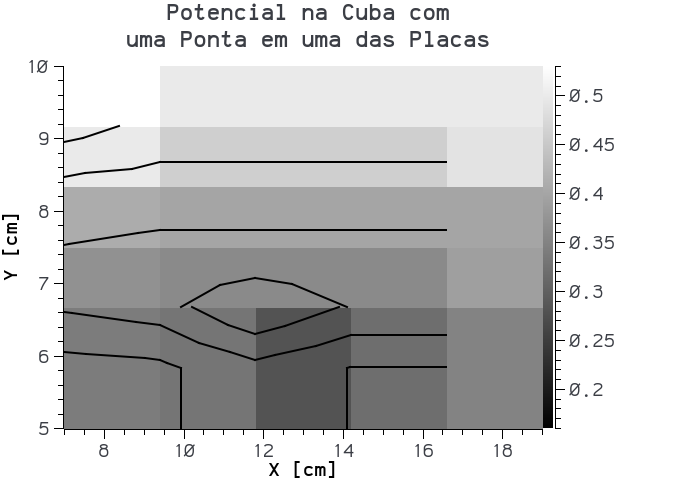
\includegraphics[width=0.6\textwidth]{contorno/limitado.png}

        \caption{Exemplos de gráfico de curvas de nível do \software}
        \label{fig:contorno:limitado}
    \end{figure}


\subsection{Simulando Curvas de Nível}

    Apesar de tudo isso, é possível simular curvas de nível com um gráfico de múltiplas variáveis. Para tanto, é preciso que os dados sejam coletados seguindo valores fixos de $z$ que significa medir as equipotenciais em valores específicos de $V$ no caso das medidas de potencial na cuba.

    \begin{figure}[htbp]
        \centering
        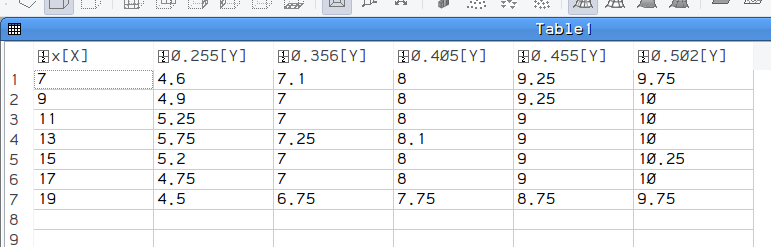
\includegraphics[width=0.6\textwidth]{contorno/1dados.png}

        \caption{Montagem dos dados de posições para cada potencial}
        \label{fig:contorno:dados}
    \end{figure}

    No \software, basta separar os valores de cada $z$ diferente em colunas próprias de $y$. A tabela deve ficar algo parecido com a da figura \ref{fig:contorno:dados}. Com isso, basta aplicar o mesmo processo de montagem do gráfico da seção \nameref{sec:multiv:juntos}.


\subsection{Opções de Formatação}

    Por padrão, o \software escolhe cores variadas para cada nível, mas é mais recomendado seguir tons variados de uma mesma cor. Para este exemplo será seguido um padrão de cores monocromáticas. Além disso, a grossura das linhas (\texttt{Line width}) foi alterada para o valor 2.

    \begin{figure}[htbp]
        \centering
        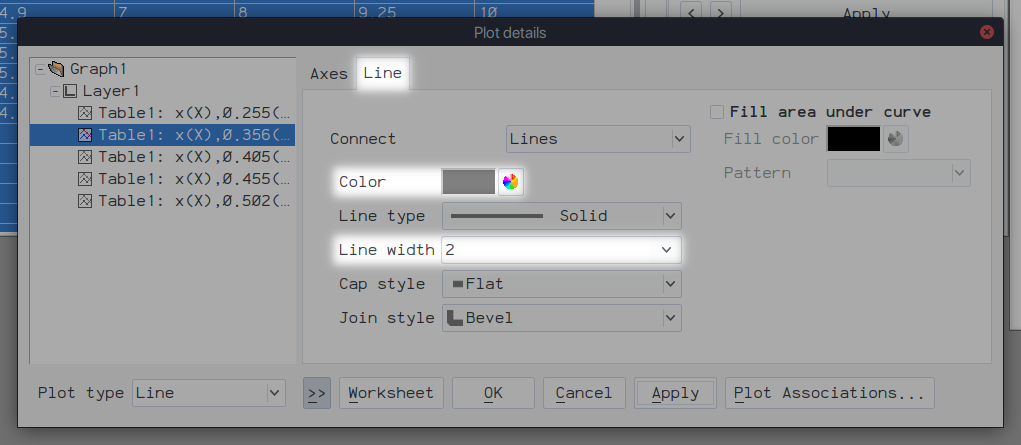
\includegraphics[width=0.6\textwidth]{contorno/2cor.png}

        \caption{Principais opções de formatação}
        \label{fig:contorno:cor}
    \end{figure}

    \begin{lembrete}
        É importante a adição de sufixos com a unidade do valor medido na legenda.
    \end{lembrete}


\subsection{Resultado}

    \begin{figure}[htbp]
        \centering
        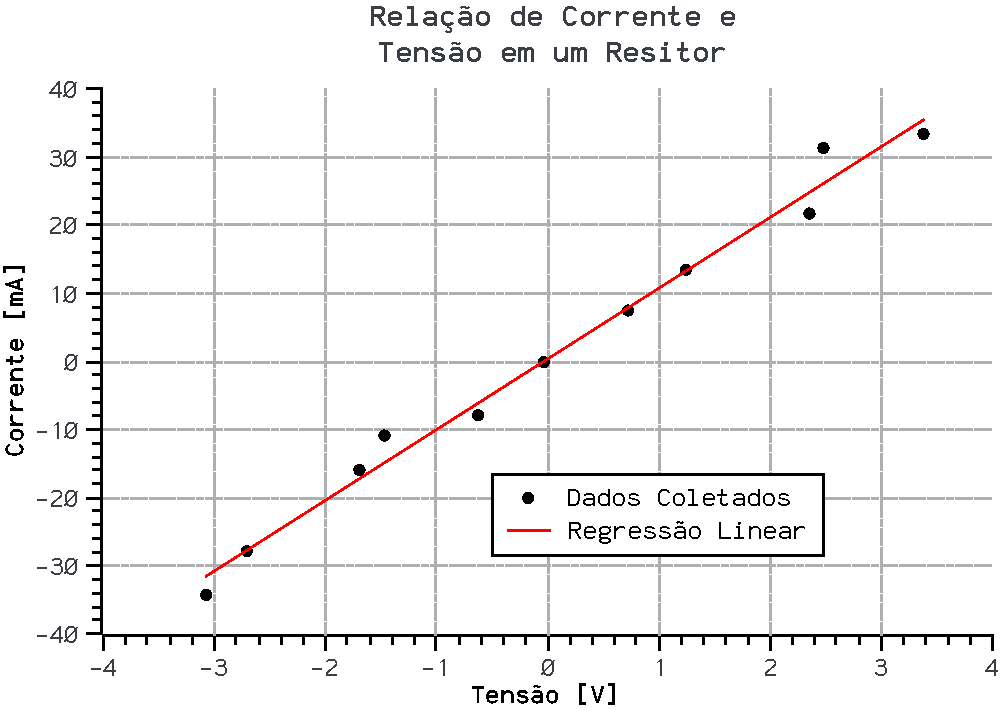
\includegraphics[width=0.6\textwidth]{contorno/resultado.pdf}

        \caption{Deformação das equipotenciais gerada pela adição de uma ponta}
        \label{fig:contorno:final}
    \end{figure}

